\subsection{A matching finite-confidence characterization}
\label{sec:exact-catalogue}
An information bound need not be tight at finite confidence. We now
characterize the catalogue optimum itself by finite optimization problems
with an explicit approximation error. Linear-programming duality and
Bayesian stopping are established tools: see \citet[Theorems 4.1--4.2]{fauss2015}
and the controlled-sensing formulation of \citet[Theorems 1--3]{lisensor2019}.
The purpose here is to connect those tools to the priced quantum catalogue,
retain every conditional error constraint, and supply certified lower and
attainable upper costs, including discrete outcomes and randomized decisions.

Return to the $K$-hypothesis catalogue of Section~\ref{sec:general-costed}.
Assume that every pair is distinguished by at least one action. Let
$C_{N,\delta}$ be the minimax cost when stopping is required after at most
$N$ actions, allowing randomization at time zero and subsequently.
Fix a baseline policy with horizon $N_0$, worst expected cost $C_0$, and
each conditional error at most $\delta_0<\delta<1/2$; write
$\Delta=\delta-\delta_0$. Such a baseline exists: a recorded mixture
assigning positive probability to every action has $A_{\max}<1$, and
Proposition~\ref{prop:catalogue-upper} gives a finite horizon.

\begin{theorem}[Finite programs converge to the exact catalogue optimum]
\label{thm:catalogue-exact}
Let $\mathcal T_N$ be the finite set of deterministic decision trees of
horizon at most $N$. For $T\in\mathcal T_N$, write $c_h(T)$ and $e_h(T)$
for its conditional expected cost and error. Then $C_{N,\delta}$ is the
value of the finite linear program
\begin{align}
 \min_{w,C}\quad &C,\notag\\
 \sum_Tw_Tc_h(T)&\leq C, &
 \sum_Tw_Te_h(T)&\leq\delta \quad(1\leq h\leq K),\label{eq:exact-tree-lp}\\
 w_T&\geq0, &\sum_Tw_T&=1.\notag
\end{align}
For every $N\geq N_0$,
\begin{equation}\label{eq:catalogue-matching}
 \frac{C_{N,\delta}}{1+C_0/(\Delta N c_{\min})}
 \leq C_{\mathcal E,\delta}^\star\leq C_{N,\delta},
 \qquad C_{N,\delta}\downarrow C_{\mathcal E,\delta}^\star.
\end{equation}
Unlike the occupation relaxation in Theorem~\ref{thm:occupation-converse},
these finite programs describe actual causal policies.
\end{theorem}
\begin{proof}
There are finitely many histories at a finite horizon. Presampling all
random decisions at those histories expresses any randomized policy as
a mixture of deterministic trees; conversely such a mixture is a policy.
This proves the program and the upper bound.

Take an admissible unrestricted policy with worst cost
$C\leq C_{\mathcal E,\delta}^\star+\epsilon$. Its stopping time $\tau$
satisfies $\Pr_h(\tau>N)\leq C/(Nc_{\min})=:\varepsilon_N$ for every $h$.
Force a decision at $N$. The truncated policy costs at most $C$ and has
each error at most $\delta+\varepsilon_N$.
At time zero, choose the baseline with probability
$w=\varepsilon_N/(\Delta+\varepsilon_N)$ and the truncated policy otherwise.
Every error of this mixture is at most $\delta$, its horizon is at most $N$,
and its worst cost is at most
\[
 (1-w)C+wC_0\leq C+
 \frac{CC_0}{\Delta Nc_{\min}}.
\]
Let $\epsilon\downarrow0$. Since the feasible classes increase with $N$,
their values decrease, and the displayed bounds force the stated limit.
\end{proof}

The finite program also has a directly evaluable dual. For $u_h,v_h\geq0$
with $\sum_hu_h=1$, define, for a nonnegative likelihood vector $l$,
\begin{align}
 W_{u,v,0}(l)&=\sum_hv_hl_h-\max_hv_hl_h,\notag\\
 W_{u,v,n+1}(l)&=\min\left\{W_{u,v,0}(l),
 \min_a\left[c_a\sum_hu_hl_h+
       \sum_yW_{u,v,n}(l\mathbin{\odot}p_a(y))\right]\right\}.
 \label{eq:likelihood-dual-dp}
\end{align}
Here $(l\mathbin{\odot}p_a(y))_h=l_hp_{h,a}(y)$.
Finite-dimensional LP duality gives
\begin{equation}\label{eq:exact-tree-dual}
 C_{N,\delta}=\max_{\substack{u\geq0,\ \sum_hu_h=1\\v\geq0}}
 \left\{W_{u,v,N}(\mathbf1)-\delta\sum_hv_h\right\}.
\end{equation}
Indeed, $u$ weights the conditional cost constraints, $v$ the conditional
errors, and backward induction minimizes the resulting weighted risk over
all trees. The finite program is feasible and bounded for $N\geq N_0$,
so strong LP duality applies. A maximizer can be sought with
$\sum_hv_h\leq C_0/\Delta$: the baseline bounds the objective above by
$C_0-\Delta\sum_hv_h$, while $v=0$ gives zero.
Thus arbitrary multipliers supply certified lower bounds, and feasible
tree mixtures supply upper bounds. Enumerating the trees can be expensive;
this characterization is not a polynomial-time algorithm in the catalogue size.

\begin{corollary}[Exponential horizon error under uniform separation]
\label{cor:catalogue-exponential}
If
\[
 a=\max_{h<k,\,a'}\sum_y\sqrt{p_{h,a'}(y)p_{k,a'}(y)}<1,
 \qquad \varepsilon_N=(K-1)a^N,
\]
then, for $N\geq N_0$,
\begin{equation}\label{eq:catalogue-exponential}
 0\leq C_{N,\delta}-C_{\mathcal E,\delta}^\star
 \leq\frac{C_0\varepsilon_N}{\Delta+\varepsilon_N}.
\end{equation}
\end{corollary}
\begin{proof}
At each living history, any randomized choice of action contracts the
pairwise affinity mass by at least the factor $a$. Killing histories that
have stopped can only reduce that mass. Consequently the affinity of the
histories still alive at time $N$ is at most $a^N$ for every pair.
Force a maximum-likelihood decision on those histories. Under $h$, an
incorrect choice of $k$ requires $P_k(z)\geq P_h(z)$, so its probability is
at most $\sum_{z\,\mathrm{alive}}\sqrt{P_h(z)P_k(z)}\leq a^N$.
Summing over $k\ne h$ gives an additional error at most $\varepsilon_N$.
Use the same baseline mixture as above. Its extra cost is at most
$C_0\varepsilon_N/(\Delta+\varepsilon_N)$, and then let the initial
policy approach the unrestricted infimum.
\end{proof}
Uniform separation is stronger than pairwise identifiability. For example,
an action in the three-state catalogue can give identical laws for two
labels; then this exponential bound does not apply, while
Theorem~\ref{thm:catalogue-exact} still does.

\subsection{An exact dual and a computable certificate in the binary case}
Call a binary catalogue \emph{reflection symmetric} if exchanging the
two labels can be implemented by cost-preserving relabellings of actions
and outcomes. Symmetrizing a policy with its reflection makes its two
costs equal to their average and its two errors equal to their average.
Thus its constrained equal-prior Bayes optimum equals its minimax optimum.

\begin{theorem}[Exact finite-confidence dual with exponential certification]
\label{thm:exact-binary-dual}
For a reflection-symmetric catalogue with maximal action affinity $a<1$,
let $V_{\lambda,N}$ be the Bellman values in~\eqref{eq:bellman} and let
$V_\lambda$ denote their unrestricted limit. For all priors $\pi$,
\begin{equation}\label{eq:bellman-exponential}
 0\leq V_{\lambda,N}(\pi)-V_\lambda(\pi)
 \leq\lambda\sqrt{\pi(1-\pi)}\,a^N.
\end{equation}
With the strictly feasible baseline above,
\begin{equation}\label{eq:binary-strong-dual}
 C_{\mathcal E,\delta}^\star
 =\max_{0\leq\lambda\leq C_0/\Delta}
       \{V_\lambda(1/2)-\lambda\delta\}.
\end{equation}
In particular, for any $\lambda\geq0$, any $N$, and any symmetric
policy with error at most $\delta$ and cost $U$,
\begin{equation}\label{eq:sharp-primal-dual}
 V_{\lambda,N}(1/2)-\lambda\delta-\frac\lambda2a^N
 \leq C_{\mathcal E,\delta}^\star\leq U.
\end{equation}
The width of this interval is an optimality certificate, not a comparison
between two heuristic policies.
\end{theorem}
\begin{proof}
Take a policy arbitrarily close to $V_\lambda(\pi)$ and truncate it at $N$,
using the posterior-optimal decision on surviving histories. Their additional
Bayes error is bounded by
\[
 \sum_{z\,\mathrm{alive}}\min\{\pi P_+(z),(1-\pi)P_-(z)\}
 \leq\sqrt{\pi(1-\pi)}
       \sum_{z\,\mathrm{alive}}\sqrt{P_+(z)P_-(z)}
 \leq\sqrt{\pi(1-\pi)}a^N.
\]
Cost decreases on truncation. Letting the approximation error vanish
proves~\eqref{eq:bellman-exponential}.

Reflection reduces the finite-horizon primal to a mixture of symmetric
trees with one average error constraint. Its LP dual is
$C_{N,\delta}=\max_{\lambda\geq0}
[V_{\lambda,N}(1/2)-\lambda\delta]$.
The baseline restricts maximizing multipliers to $[0,C_0/\Delta]$,
as in~\eqref{eq:exact-tree-dual}. On this compact interval,
\eqref{eq:bellman-exponential} gives uniform convergence. Passing to
the limit, using Theorem~\ref{thm:catalogue-exact}, proves
\eqref{eq:binary-strong-dual}. Finally any feasible policy has cost at least
$V_\lambda(1/2)-\lambda\delta$, which proves the lower side of
\eqref{eq:sharp-primal-dual}; the proposed policy supplies the upper side.
\end{proof}
This argument includes discrete likelihood ratios. It does not assume
differentiability of the value in $\lambda$ or that one deterministic
threshold achieves the desired error exactly. Mixing policies on opposite
sides of a kink can be necessary.

\subsection{An exact measurement-price transition}
\label{sec:sharp-price}
A second route to a sharp converse is to simulate one experiment with
another. This is the decision-theoretic comparison principle associated
with \citet{blackwell1953}, now with the simulation cost included.

\begin{lemma}[Simulation gives cost dominance]\label{lem:cost-simulation}
Suppose a new action can be simulated with an existing catalogue, producing
exactly its conditional output law under every hypothesis, at expected
cost at most $c_{\rm sim}$ under every hypothesis. If its charged price
is at least $c_{\rm sim}$, adding the action cannot decrease any
finite-confidence minimax expected cost.
\end{lemma}
\begin{proof}
Replace each invocation of the new action by a fresh simulation, exposing
only its reported output to the original controller. Conditional on every
external history, the output law is unchanged and expected cost does not
increase. Conditional expectation and summation over invocations prove
the total-cost comparison for every finite-cost policy. The original
catalogue is a subclass of the enlarged one, so the two infima are equal.
\end{proof}

Consider the full-rank, noncommuting states
\begin{equation}\label{eq:sharp-states}
 \rho_\pm=\frac12\left(I+\frac{59}{100}X\pm\frac45Y\right).
\end{equation}
Their squared Bloch radius is $9881/10000<1$.
Action $Y$ measures $Y$ at price $c_Y=1$.
Action $E$ has price $c_E=\kappa>0$ and POVM
\begin{equation}\label{eq:sharp-effects}
 E_\pm=\frac{17}{50}
   \left(I-\frac{470}{1003}X\pm\frac{15}{17}Y\right),
 \qquad E_0=\frac8{25}I+\frac{94}{295}X.
\end{equation}
The effects sum to $I$ and are positive: for $E_\pm$ the squared Bloch
length is $(470/1003)^2+(15/17)^2<1$, while $8/25>94/295$ for $E_0$.
Under the positive label, the observation laws are exactly
\begin{equation}\label{eq:sharp-laws}
 p_{+,Y}=(9/10,1/10),\qquad
 p_{+,E}=(243/500,3/500,127/250).
\end{equation}
The negative label exchanges the first two probabilities.
These are single-copy quantum measurements with explicitly assigned
prices; no implementation-time claim is implicit in choosing those prices.

\begin{theorem}[Sharp universal price threshold $6/5$]
\label{thm:sharp-price}
For this two-action catalogue and every $0<\delta<1/2$,
\begin{equation}\label{eq:sharp-price-threshold}
 \kappa\geq\frac65\quad\Longrightarrow\quad
 C_{\{Y,E\},\delta}^\star(\kappa)=C_{\{Y\},\delta}^\star.
\end{equation}
The threshold is sharp: for each $0<\kappa<6/5$, strict improvement
holds for all sufficiently small $\delta$. More precisely,
\begin{equation}\label{eq:sharp-price-limit}
 \lim_{\delta\downarrow0}
 \frac{C_{\{Y,E\},\delta}^\star(\kappa)}{C_{\{Y\},\delta}^\star}
 =\min\{1,5\kappa/6\}.
\end{equation}
At equal prices the limiting cost reduction is therefore $1/6$.
\end{theorem}
\begin{proof}
With probability $3/5$, take two independent $Y$ samples; report $+$
if both are positive, $-$ if both are negative, and $0$ otherwise.
With probability $2/5$, report $0$ without sampling. Under the positive
label this gives
\[
 \Pr(+)=(3/5)(9/10)^2=243/500,\qquad
 \Pr(-)=(3/5)(1/10)^2=3/500;
\]
the remaining probability is $127/250$. The expected cost is exactly
$2(3/5)=6/5$ under either label. Lemma~\ref{lem:cost-simulation}
proves the all-confidence equality.

The directed divergences agree in both directions and satisfy
\[
 d_Y=\frac45\log9,\qquad
 d_E=\frac{12}{25}\log81=\frac65d_Y.
\]
The stopped-KL converse lower-bounds cost by
$k_\delta/\max\{d_Y,d_E/\kappa\}$.
Repeating the maximizing action and using a likelihood-ratio test
achieves the same leading coefficient: its increments are bounded and
its expected cost is at most
$[\log(1/\delta)+L]/\max\{d_Y,d_E/\kappa\}$ for a fixed overshoot bound $L$.
Divide by $\log(1/\delta)$ and compare with the one-action coefficient
$1/d_Y$. This gives~\eqref{eq:sharp-price-limit} and strict improvement
below $6/5$ at sufficiently high confidence.
\end{proof}
The result identifies a universal dominance price for this specified
catalogue. It does not claim that the finite-confidence onset of a gain
occurs at the same price for every $\delta$, or that these two readouts
exhaust all POVMs.

\subsection{The complete confidence--price frontier}
\label{sec:exact-price-frontier}
The example belongs to a solvable family. Let $0<s<1$, $0<\alpha\leq1$,
$p=(1+s)/2$, $q=(1-s)/2$, and consider the reflected laws
\begin{equation}\label{eq:lattice-family}
 p_{+,Y}=(p,q),\qquad
 p_{+,E}=(\alpha p^2,\alpha q^2,1-\alpha(p^2+q^2)),
 \qquad p_{-,a}=\text{reflection of }p_{+,a}.
\end{equation}
The preceding example has $s=4/5$, $\alpha=3/5$.
The prices remain $1$ and $\kappa$. Simulation with probability $\alpha$
and two $Y$ samples proves dominance at $\kappa\geq2\alpha$; the
information-rate calculation gives limiting cost ratio
$\min\{1,\kappa/(2\alpha)\}$.
The integer likelihood process has more structure than these asymptotics:
its parity records the number of $Y$ observations and closes the
finite-confidence lower bound exactly.
For integers $b\geq0$, put
\begin{equation}\label{eq:barrier-points}
 R=p/q,\qquad \epsilon_b=\frac1{1+R^b},\qquad
 g_b=b(1-2\epsilon_b).
\end{equation}
\begin{equation}\label{eq:barrier-costs}
 K_b(\kappa)=
 \begin{cases}
 \dfrac{\kappa}{2\alpha s}g_b+
       \left(1-\dfrac{\kappa}{2\alpha}\right)\mathbf1_{\{b\text{ odd}\}},
       &0<\kappa\leq2\alpha,\\[3pt]
 \dfrac1s g_b,&\kappa\geq2\alpha.
 \end{cases}
\end{equation}
The two expressions agree at $2\alpha$, and $K_0=0$.

\begin{theorem}[Exact finite-confidence and price frontier]
\label{thm:exact-price-frontier}
For the entire family~\eqref{eq:lattice-family}, all $\kappa>0$,
and all $0<\delta<1/2$,
\begin{align}
 C_{\{Y,E\},\delta}^\star(\kappa)
 &=\min_{\substack{w_b\geq0,\ \sum_bw_b=1\\
                    \sum_bw_b\epsilon_b\leq\delta}}
                       \sum_bw_bK_b(\kappa)\label{eq:exact-price-primal}\\
 &=\max_{\lambda\geq0}
       \left\{\min_{b\geq0}[K_b(\kappa)+\lambda\epsilon_b]
                   -\lambda\delta\right\}.\label{eq:exact-price-dual}
\end{align}
The minimum is attained by a mixture of at most two finite barriers.
Here $z$ is log likelihood divided by $\log R$.
For $\kappa\leq2\alpha$, an even barrier uses $E$ until $z=\pm b$;
an odd barrier takes one $Y$ observation and then uses $E$ until
$z=\pm b$. Barrier zero stops immediately with a fair guess.
For $\kappa\geq2\alpha$, use $Y$ until $z=\pm b$ instead.
The error of barrier $b$ is exactly $\epsilon_b$ and its cost is $K_b$.
\end{theorem}
\begin{proof}
By reflection we may restrict to symmetric policies and posterior-optimal
terminal decisions. Let $z$ be the signed log likelihood divided by $\log R$,
and let $N_Y,N_E$ count the two actions. Under the positive label their
conditional mean increments are $s$ and $2\alpha s$, respectively. Finite
expected cost implies finite expected action count, so bounded increments
justify the stopped drift identity
\[
 \E_+z_\tau=s\E_+N_Y+2\alpha s\E_+N_E.
\]
If $\overline\E$ denotes expectation under equal priors, symmetry and
the terminal likelihood ratio $R^{z_\tau}$ give
\[
 \E_+z_\tau=\overline\E g_{|z_\tau|},\qquad
 \E_+N_Y=\overline\E N_Y,\qquad
 \Pr_+(\text{error})=\overline\E\epsilon_{|z_\tau|}.
\]
Only $Y$ changes parity. Hence, pathwise,
$N_Y\geq\mathbf1_{\{|z_\tau|\text{ odd}\}}$.
For $\kappa\leq2\alpha$ the coefficient of $N_Y$ in the cost identity is
nonnegative, and therefore
\begin{align*}
 \E_+(N_Y+\kappa N_E)
 &=\frac{\kappa}{2\alpha s}\overline\E g_{|z_\tau|}
       +\left(1-\frac{\kappa}{2\alpha}\right)\overline\E N_Y\\
 &\geq\overline\E K_{|z_\tau|}(\kappa).
\end{align*}
The distribution of $|z_\tau|$ thus supplies feasible weights in
\eqref{eq:exact-price-primal}, proving its lower bound.

For an even positive barrier, $E$ preserves even parity and hits $\pm b$
without overshoot. For an odd barrier the initial $Y$ step selects odd
parity, after which $E$ again hits $\pm b$ exactly. These finite-state
absorbing chains have finite mean duration, since every nonabsorbing
state has a positive-probability path of bounded length to a boundary.
Their terminal likelihood ratios are $R^{\pm b}$ and reflection makes
the two errors equal, giving error $\epsilon_b$. Their numbers of $Y$
observations are exactly zero or one, so they attain equality in the
cost bound. Mixtures attain the corresponding convex combinations.

For $\kappa\geq2\alpha$, the simulation described above reduces the problem
to $Y$ alone. Its stopped drift identity gives cost
$(1/s)\overline\E g_{|z_\tau|}$, attained by each integer $Y$ barrier.
This proves the analogous lower and upper constructions.

For completeness, minimize cost plus $\lambda$ times error. The same
argument proves directly
$V_\lambda(1/2)=\min_b[K_b+\lambda\epsilon_b]$.
The minimum is attained at finitely many barriers, since $K_b$ grows
linearly in $b$. Theorem~\ref{thm:exact-binary-dual} gives
\eqref{eq:exact-price-dual} and a finite maximizing multiplier.
For $\delta<1/2$ a maximizer is positive: near $\lambda=0$ the unique
minimizing barrier is zero, so the dual initially increases with slope
$1/2-\delta$. At a maximizing multiplier, the slopes of the active
affine functions bracket $\delta$. Two active barriers, or one with
$\epsilon_b=\delta$, can therefore be mixed to have error exactly
$\delta$ and cost equal to the dual value. This proves attainment and
the two-barrier assertion.
\end{proof}

The two barriers need not be adjacent. Cheap $E$ readout can remove odd
barriers from the lower convex envelope; restricting the calculation
to adjacent likelihood thresholds would then be wrong.
For rational $s,\alpha,\kappa,\delta$, the barrier costs, mixing weights,
dual multiplier, and optimal value can all be certified with exact
rational arithmetic. To certify a candidate dual intercept $H$, it is
enough to check finitely many $b$: for $b\geq1$,
\begin{equation}\label{eq:barrier-tail-cutoff}
 K_b(\kappa)\geq
 \begin{cases}[\kappa/(2\alpha)]b,&\kappa\leq2\alpha,\\ b,&\kappa\geq2\alpha.
 \end{cases}
\end{equation}
Thus barriers beyond $H/\min\{\kappa/(2\alpha),1\}$ cannot improve the
supporting line. This is an exact finite termination certificate,
not an arbitrarily chosen threshold cutoff.

\begin{proposition}[Which lattice laws admit a single-qubit readout?]
\label{prop:lattice-realizability}
Let $0<s<1$, $x>0$, $x^2+s^2\leq1$, and
$\rho_\pm=(I+xX\pm sY)/2$. Put $t=(1+s^2)/2$.
The $E$ laws in~\eqref{eq:lattice-family} are realized by a three-outcome
POVM on one copy if and only if
\begin{equation}\label{eq:lattice-realizability}
 x^2\geq1-t^2,\qquad
 0<\alpha\leq
 \alpha_{\max}(x,s):=
 \frac{t+\sqrt{t^2-(1-x^2)}}{1+x}.
\end{equation}
At the pure-state boundary $x=\sqrt{1-s^2}$,
$\alpha_{\max}=1/(1+x)$. The attainable sharp price threshold of the
family can therefore reach $2/(1+x)$ on that boundary.
\end{proposition}
\begin{proof}
Average any realizing POVM with its reflection under conjugation by $X$.
Its effects have the form
$E_\pm=(wI-AX\pm\alpha Y\pm dZ)/2$ and
$E_0=(1-w)I+AX$. The $Z$ coefficient does not affect the stated laws;
setting it to zero only improves positivity. Matching probabilities gives
$w-xA=\alpha t=:q_0$. Positivity requires
\[
 A^2+\alpha^2\leq w^2,\qquad |A|\leq1-w.
\]
Since $q_0<\alpha\leq w$, necessarily $A>0$.
Substituting $w=q_0+xA$ reduces feasibility to
\[
 0\leq A\leq\frac{1-q_0}{1+x},\qquad
 f(A):=(q_0+xA)^2-A^2-\alpha^2\geq0.
\]
The concave quadratic has its unconstrained maximum at
$A_*=q_0x/(1-x^2)$. If $q_0\leq1-x$, this point is feasible and
$f(A_*)\geq0$ exactly when $t^2\geq1-x^2$.
If $q_0>1-x$, the maximum occurs at the right endpoint and is
nonnegative exactly when
\[
 (1+x)\alpha^2-2t\alpha+(1-x)\leq0.
\]
Combining the two cases gives~\eqref{eq:lattice-realizability}; the
larger quadratic root is $\alpha_{\max}$. Conversely, choose
$A=\min\{A_*,(1-q_0)/(1+x)\}$ and $w=q_0+xA$ to construct a POVM
whenever these conditions hold. At the pure boundary the square root
in~\eqref{eq:lattice-realizability} is $x^2/2$, yielding $1/(1+x)$.
\end{proof}
Thus the exact frontier is not merely a formal pair of classical channels:
an explicit region of qubit geometry realizes it. Full-rank interior
states are included. Nevertheless the optimality claim remains relative
to the two declared readouts, not to all possible POVMs on those states.

\subsection{Certified optimal costs without posterior-grid interpolation}
\label{sec:sharp-certificates}
For~\eqref{eq:sharp-laws}, log likelihood divided by $\log9$ is an integer
$z$. A $Y$ observation changes it by $\pm1$; an $E$ observation by
$\pm2$ or $0$. The posterior is exactly $9^z/(1+9^z)$.
At horizon $N$ there are only $O(N^2)$ reachable time--likelihood states,
so backward induction needs no interpolation or continuous-grid search.
The action affinities are $3/5$ and $77/125$, respectively.

The script first computes the two-barrier optimum and verifies every
relevant dual inequality with exact rational arithmetic, including the
tail cutoff~\eqref{eq:barrier-tail-cutoff}. Decimal displays are rounded
outward. Independently, it encloses the full two-action Bellman recursion
at horizon $N=96$ and checks its value against the exact barrier dual
using~\eqref{eq:bellman-exponential}. Thus the constructive formula is
also checked against a solver that allows all adaptive action choices.
Neither a posterior-grid tolerance nor a guessed threshold cutoff is
used to certify the reported optimum.

\begin{table}[htbp]
\centering\small
\begin{tabular}{rrrrr}
\toprule
$\kappa$ & $\delta$ & Barriers & Lower display & Upper display\\
\midrule
0.5 & 0.05 & $(0,2)$ & 0.9375000000 & 0.9375000000\\
0.5 & 0.01 & $(2,4)$ & 1.2106481481 & 1.2106481482\\
0.5 & 0.0001 & $(4,6)$ & 2.4455175468 & 2.4455175469\\
1 & 0.05 & $(1,2)$ & 1.5879629629 & 1.5879629630\\
1 & 0.01 & $(2,3)$ & 2.2861111111 & 2.2861111112\\
1 & 0.0001 & $(4,5)$ & 4.6331807270 & 4.6331807271\\
1.2 & 0.05 & $(1,2)$ & 1.8194444444 & 1.8194444445\\
1.2 & 0.01 & $(2,3)$ & 2.7027777777 & 2.7027777778\\
1.2 & 0.0001 & $(4,5)$ & 5.4824605624 & 5.4824605625\\
\bottomrule\end{tabular}
\caption{Exact catalogue minimax costs for the noncommuting states in
\eqref{eq:sharp-states}. Each displayed interval encloses an exactly certified rational optimum;
its width is at most $10^{-10}$, solely from decimal display rounding. Barrier policies attain
the exact value. The independent interval Bellman check at horizon 96 agrees within $10^{-12}$.}
\label{tab:sharp-costs}
\end{table}


The price
$\kappa=6/5$ rows also certify the $Y$-only optimum by
Theorem~\ref{thm:sharp-price}; these are not merely lower bounds on a
fixed-threshold implementation. At equal prices the examples demonstrate
a finite-confidence readout benefit against the entire adaptive $Y$-only
class, including randomized stopping rules. The exact rational values
and the independent Bellman enclosures accompany the source.

\begin{figure}[htbp]
 \centering
 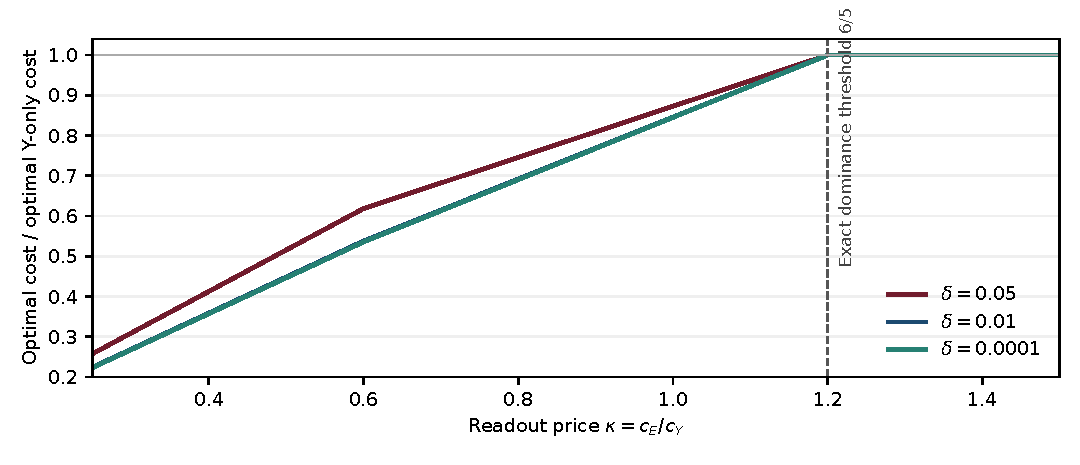
\includegraphics[width=.92\linewidth]{sharp_price_frontier.pdf}
 \caption{The exact confidence--price frontier of
 Theorem~\ref{thm:exact-price-frontier}, divided by the optimal $Y$-only
 cost. Every plotted price is checked by an exact rational primal--dual
 certificate. Lines join those samples; the equality plateau for
 $\kappa\geq6/5$ is proved for all prices, not inferred from the plot.
 The comparison concerns the two declared quantum readouts.}
 \label{fig:sharp-price-frontier}
\end{figure}

\paragraph{What is established and what is new in this development.}
The LP/Bellman method and controlled measurement selection have prior
theory \citep{fauss2015,lisensor2019}; the comparison-of-experiments principle
is classical \citep{blackwell1953}. The developments established here are
the explicit horizon-to-minimax bounds for the stated catalogue, the
parity-based exact confidence--price frontier, and its exactly realized
$6/5$ transition with rational optimality certificates. These supply a sharp, reproducible
characterization inside a declared model. They do not establish a new
general computational-complexity separation or priority over all work on
sequential experimental design.
